\chapter{Bases de numération}
\introduction{Partons sur de bonnes bases.}


On note $\N$ l'ensemble des \textit{entiers naturels} : $\N=\lbrace 0;1;2;\ldots\rbrace$.\\

Nous avons l'habitude d'utiliser la base 10 pour représenter les entiers naturels, c'est-à-dire qu'on utilise 10 symboles, appelés \textit{chiffres}
pour les écrire : 0, 1, 2, \ldots, 9.
Or il n'en a pas toujours été ainsi :
\begin{itemize}
    \item 	au \textsc{I}\er millénaire av. J.-C., les Babyloniens utilisaient la base soixante pour mesurer le temps et les angles ;
    \item 	durant le \textsc{I}\er millénaire, les Mayas et les Aztèques se servaient de la base vingt (et d'ailleurs en France, 80 se lit «
          quatre-vingts » ) ;
    \item 	entre le \textsc{vii}\eme et le \textsc{xv}\eme siècle, les astronomes arabes utilisaient la base cent cinquante pour élaborer des tables
          permettant de trouver la position d'un astre dans le ciel à un moment donné.
\end{itemize}
De nos jours, en Informatique, on utilise beaucoup la base deux, dite \textit{binaire} et la base seize, appelée \textit{hexadécimale}.\\
L'objectif de ce chapitre est de donner les méthodes permettant d'écrire un entier naturel dans une base donnée, plus précisément dans les bases 2,
10 et 16. Nous verrons également comment passer facilement du binaire à l'hexadécimal et vice-versa.

\section{\'Ecriture binaire d'un entier naturel}
\subsection{Pourquoi le binaire ?}


\floatpictureleft{0.2}{bases/img/joke1}{
Pour simplifier, disons qu'au niveau le plus «  bas  » {} d'un ordinateur, se trouvent des (millions de) transistors
qui jouent chacun un rôle d'interrupteur. De multiples points de l'ordinateur peuvent alors être soumis à une tension
(état 1) ou non (état 0).
En considérant 2 de ces points, on voit que l'état de ce système peut être 00, 01, 10 ou 11. Cela fait 4 possibilités
et le binaire est né !
}
\subsection{Comprendre l'écriture en base 2}

Puisqu'il n'y a que deux chiffres en binaire, compter est simple mais nécessite rapidement plus de chiffres qu'en base
10 :\\

\begin{center}
    \tabstyle[UGLiBlue]
    \begin{tabular}{CCCCCCCCCCC}
        
        \ccell \'Ecriture décimale & 0 & 1 & 2  & 3  & 4   & 5   & 6   & 7   & 8    & \dots \\
        
        \ccell\'Ecriture binaire   & 0 & 1 & 10 & 11 & 100 & 101 & 110 & 111 & 1000 & \dots \\
    \end{tabular}
\end{center}

\begin{notation}
    On écrira $(11)_{10}$ pour insister sur le fait qu'on parle du nombre 11 \textit{en base 10}, et $(11)_2$ pour dire que c'est une écriture
    binaire.\\
    Lorsque ce n'est pas précisé cela veut dire que l'écriture est en base 10.\\
    Ainsi $(11)_2=3$, et de même, $(111)_2=7$.\\
\end{notation}


Tout entier naturel admet une unique écriture décimale (c'est-à-dire en base 10), il en va de même en binaire:
\begin{propriete}[ : écriture binaire d'un entier naturel]
    Tout entier naturel possède une unique écriture en base 2, dite \textit{écriture binaire}.
    Plus précisément, soit $n\in\N$, alors il existe un unique entier $k\in\N$ et $k+1$ nombres $a_i$, uniques et valant 0
    ou 1 et tels que $$n=a_02^0+a_12^1+\ldots+a_k2^k$$
    ce qui s'écrit aussi
    $$n=\sum_{i=0}^ka_i2^i$$
\end{propriete}
\begin{exemple}
    Lorsqu'on regarde le tableau précédent, on voit que $6=(110)_2$.\\Cela s'interprète ainsi :\\
    
    \tabstyled
    \begin{tabular}{CCCC}
        \ccell Chiffre binaire & 1     & 1     & 0     \\
        \ccell Valeur          & $2^2$ & $2^1$ & $2^0$ \\
    \end{tabular}\ \ \ et on obtient $6=0\times 2^0+1\times 2^1+1\times 2^2$.
\end{exemple}

\begin{methode}[ 1 : passer de la base 2 à la base 10]
    Que vaut $(11101)_2$ ?
    \begin{center}
        \alternaterowcolors[UGLiPurple]
        \begin{tabular}{CCCCCC}
            \ccell Chiffre binaire & 1     & 1     & 1     & 0     & 1     \\
            \ccell Valeur          & $2^4$ & $2^3$ & $2^2$ & $2^1$ & $2^0$ \\
        \end{tabular}
    \end{center}
    \begin{tabbing}
        $(11101)_2$	\= 	$=1\times 2^4+1\times 2^3+1\times 2^2+0\times 2^1+1\times 2^0$	\\
        \>	$=16+8+4+1$	\\
        \>	$=29$
    \end{tabbing}\nopagebreak
\end{methode}
\begin{exercice}
    \begin{enumerate}
        \item Donner l'écriture décimale des onze premières puissances de deux.
        \item Donner l'écriture décimale de $(1101)_2$ et $(1\ 1010)_2$
    \end{enumerate}
    
\end{exercice}

\begin{methode}[ 2 : passer de la base 10 à la base 2]
    Comprenons ce que veut dire une écriture décimale :
    \begin{tabbing}
        $203$	\= 	$=200+3$	\\
        
        \>	$=2\times 10^2+0\times 10^1+3\times 10^0$
    \end{tabbing}
    Faisons la même chose en base 2 :
    \begin{tabbing}
        $203$	\= 	$=128+64+8+2+1$	\\
        
        \>	$=2^7+2^6+2^3+2^1+2^0$	\\
        
        \>	$=1\times 2^7+1\times 2^6+0\times 2^5 + 0\times 2^4 +1\times 2^3+0\times 2^2 + 1\times
            2^1+1\times 2^0$	\\
        
        \> $=(11001011)_2$
    \end{tabbing}
    Cette méthode est pratique quand l'entier est petit et que l'on connaît bien les premières puissances de deux.\\
    Quand ce n'est pas le cas, une autre méthode (la méthode 3) peut être employée.
    
\end{methode}
\'Evidemment, \textsc{Python} connait le binaire et travaille avec des valeurs entières de type \mintinline{python}{int} (\textit{integer} veut dire « entier » en Anglais, pour plus de précisions, voir le chapitre \ref{ch:valeurs}, partie \ref{sec:int} ).\\
Voici comment écrire un \mintinline{python}{int} en binaire et comment obtenir l'écriture
binaire d'un \mintinline{python}{int}.
\begin{pyc}
    \begin{minted}{python}
        >>> 0b11001011 # faire précéder le nombre de 0b
        203
        >>> bin(29)
        '0b11101'
    \end{minted}
\end{pyc}
\begin{exercice}[]
    Appliquer la méthode 2 pour donner les écritures binaires des nombres suivants.
    \begin{enumalph}
        \item 6 ;
        \item 26 ;
        \item 126 ;
        \item 1026.
    \end{enumalph}
\end{exercice}
\subsection{Un algorithme pour déterminer l'écriture binaire d'un entier naturel}
\begin{methode}[ 3 : les divisions successives]
    Voici comment on trouve les chiffres de l'écriture \textit{décimale} de 203 :\\
    
    On divise 203 par 10, cela fait 20, il reste 3, c'est le chiffre des unités.\\
    On recommence avec 20, on le divise par 10, cela fait 2, reste 0, chiffre des dizaines.\\
    On continue, on divise 2 par 10, cela fait 0, reste 2, chiffre des des centaines.\\
    Puisqu'on a trouvé un quotient de 0, on s'arrête.\\
    On peut écrire cela simplement :
    $$\division[10]{203}$$
    Voici maintenant comment on trouve son écriture binaire. On procède comme en base 10 mais en divisant par 2 :
    $$\division[2]{203}$$
    
    On a donc successivement établi :
    \begin{tabbing}
        203	\= 	$=101\times 2 +1$	\\
        \>	$=(50\times 2 +1)\times 2+1  $	\\
        \>	$=((25\times 2 +0)\times 2 +1)\times 2+1  $	\\
        \>	$=(((12\times 2 +1)\times 2 +0)\times 2 +1)\times 2+1  $	\\
        \>	$=((((6\times 2 +0)\times 2 +1)\times 2 +0)\times 2 +1)\times 2+1  $	\\
        \>	$=(((((3\times 2 +0)\times 2 +0)\times 2 +1)\times 2 +0)\times 2 +1)\times 2+1  $	\\
        \>	$=((((((1\times 2 +1)\times 2 +0)\times 2 +0)\times 2 +1)\times 2 +0)\times 2 +1)\times 2+1  $	\\
        
        \>	$=1\times 2^7+1\times 2^6+0\times 2^5 + 0\times 2^4 +1\times 2^3+0\times 2^2 + 1\times 2^1+1\times
            2^0$\\
        \> $=(11001011)_2$
    \end{tabbing}
    Cette succession d'égalités n'est (heureusement) pas à écrire à chaque fois.
\end{methode}

\begin{exercice}[]
    Utiliser la méthode 3 pour retrouver les écritures binaires de l'exercice précédent.
\end{exercice}
Les trois méthodes précédentes se programment facilement et la dernière est de loin la plus courte à écrire.

\subsection{Vocabulaire}

\floatpictureleft{0.4}{bases/img/bitjoke}{
Un chiffre décimal peut être 0, 1, 2, 3, 4, 5, 6, 7, 8 ou 9.\\
Un chiffre binaire peut être seulement 0 ou 1. En Anglais, \textit{chiffre binaire} se traduit par \textit{binary digit},
que l'on abrège en \textit{bit}. On garde cette dénomination en Français.\\

Le bit est «  le plus petit morceau d'information numérique  » {}.\\

Pour les écrire, on regroupe les chiffres décimaux par paquets de 3, comme dans \np{1230014} par exemple.
En binaire on groupe les bits par 4, on écrira donc $17=\left(1\ 0001\right)_2$.
}\medskip\par

La plupart du temps, en machine, les bits sont groupés par 8 (deux paquets de 4). Un tel paquet s'appelle un \textit{octet}, et on écrit donc des \textit{mots binaires} de longueur 8 tels que $0000\ 0011$ : l'octet représente ici le nombre 3. Les bits à zéros ne sont pas inutiles.\\

Lorsqu'on considère un nombre écrit en binaire, on parle souvent de \textit{bit de poids fort} et de
\textit{bit de poids faible} pour parler respectivement du bit associé à la plus grande puissance de 2, et du bit
d'unités.\\
Considérons l'octet $(0010\ 0101)_2$. Son bit de poids fort est 0, son bit de poids faible est 1.

\section{\'Ecriture hexadécimale d'un entier naturel}

La base «  naturelle  » {} de l'informatique est la base 2, mais elle n'est pas très pratique car elle donne lieu à
des écritures trop longues.
La base 10 nous paraît bien meilleure parce que nous avons l'habitude de l'utiliser, mais elle ne fait pas bon ménage
avec la base 2 : il n'y a pas de méthode simple pour passer du décimal au binaire, et vice versa.\\
La base 16, ou base \textit{hexadécimale}, est en revanche très adaptée à l'écriture des paquets de 4 bits, et par
extension à celle des octets et autres écritures binaires.\\

En hexadécimal, on dispose de 16 chiffres : 0, 1, 2, 3, 4, 5, 6, 7, 8, 9, A, B, C, D, E et F.

\begin{propriete}[ : écriture binaire d'un entier naturel]
    Tout entier naturel possède une unique écriture en base 16, dite \textit{écriture hexadécimale}.
    Plus précisément, soit $n\in\N$, alors il existe un unique entier $k\in\N$ et $k+1$ nombres $a_i$, uniques et valant 0, 1, 2, \ldots, ou F et tels
    que $$n=a_016^0+a_16^1+\ldots+a_k16^k$$
    ce qui s'écrit aussi
    $$n=\sum_{i=0}^ka_i16^i$$
\end{propriete}

\begin{remarque}
    On a vu une propriété similaire en base 2 et en fait elle est valable \textit{dans toutes les bases}  $b$ (où $b$ est un entier naturel supérieur ou
    égal à 2). Cela justifie par exemple l'utilisation de la base 20 ou de la base 150.
\end{remarque}

Les méthodes que l'on a vu en base 2 et 10 se transposent en base 16.
\begin{methode}[ 4 : passer de la base 16 à la base 10]
    Déterminons l'écriture décimale de $(D4A)_{16}$ :
    \begin{tabbing}
        $(D4A)_{16}$  	\= $=13\times 16^2 + 4\times 6 + 10\times 16^0$	 car D vaut 13 et A vaut 10.\\
        \>	$=3402$
    \end{tabbing}
\end{methode}
\begin{methode}[ 5 : passer de la base 10 à la base 16]
    Déterminons maintenant l'écriture hexadécimale de 503:
    $$\division[16]{503}$$
    
    $503 = 31 \times 16 + \underline{7}$.\\
    
    $31 = 1\times 16 + \underline{15}$ et 15 s'écrit $\underline{F}$.\\
    
    $1 = {\boldmath 0}\times 16 + \underline{1}$ et on arrête car le quotient est nul.\\
    
    $503=(1F7)_{16}$.\\
    
\end{methode}
\begin{figure}[H]
    \begin{center}
        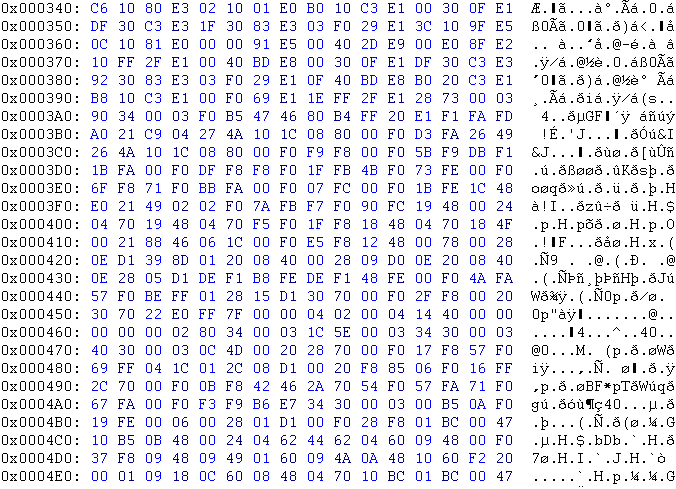
\includegraphics[width=12cm]{bases/img/hex.png}\\
        \caption*{Un éditeur hexadécimal montre le contenu d'un fichier, d'un disque dur, ou de la RAM d'un ordinateur. La première colonne indique l'adresse,
            puis 16 octets écrits en hexadécimal et enfin les caractères correspondants.}
    \end{center}
\end{figure}
\section{Hexadécimal et binaire : un mariage heureux}
Le grand avantage qu'apporte l'hexadécimal s'illustre facilement :

\begin{methode}[ 6 : passer de la base 2 à la base 16]
    \begin{tabbing}
        $(101101000011101)_2$	\=	$=(0101\ 1010\ 0001\ 1101)_2$\\
        \>	$=\left(\underbrace{0101}_5\ \underbrace{1010}_A\ \underbrace{0001}_1\ \underbrace{1101}_D\right)_2$\\
        \>	$=(5A1D)_{16}$
    \end{tabbing}
\end{methode}

\begin{methode}[ 7 : passer de la base 16 à la base 2]
    $(F7B)_{16}=\left(\underbrace{1111}_F\ \underbrace{0111}_7\ \underbrace{1011}_B\right)_2$
\end{methode}
\begin{figure}
    \begin{center}
        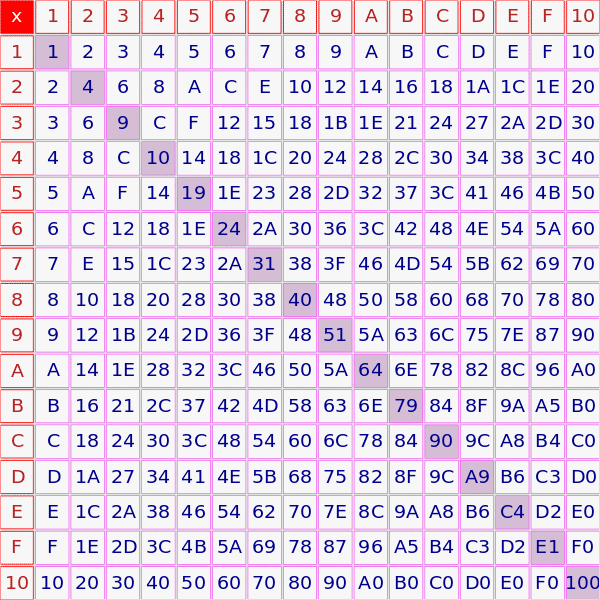
\includegraphics[width=10cm]{bases/img/hexmult.png}\\
        \caption*{Table de multiplication hexadécimale.}
    \end{center}
\end{figure}


\section{Additions}

On pose l'opération à la main : c'est la même chose qu'en base 10.
\subsection*{En base 2}
La seule différence avec la base 10 c'est que deux 1 donnent $(2)_{10}$ donc $(10)_2$, donc un zéro et une retenue de 1.
Quand il y a deux 1 et une retenue de 1 en plus, cela donne $(3)_{10}$ donc $(11)_2$, donc un 1 et une retenue de 1.

\tabulardefault
\begin{exemple}[]
    \begin{center}
        \begin{tabular}{ccccccccc}
              &   &   & $_1$ & $_1$ & $_1$ &   &   &   \\
              & 1 & 1 & 0    & 1    & 0    & 1 & 0 & 1 \\
            + &   &   &      & 1    & 1    & 1 & 0 & 0 \\
            \hline
            = & 1 & 1 & 1    & 1    & 0    & 0 & 0 & 1 \\
        \end{tabular} \\[2em]
    \end{center}
\end{exemple}

\subsection*{En base 16}

C'est encore la même chose. Il faut bien se souvenir de la valeur de A, B, C, D, E et F.\\
Ajouter 8 et 3 ne provoque pas de retenue puisque $8+3=11$ et que $11$ est $B$ en base 16.\\
Dès que l'addition de 2 chiffres dépasse 15, il y aura une retenue : par exemple 9 et A donnent $(19)_{10}$, donc $(13)_{16}$. Ainsi on note 3 et une retenue de 1.

\begin{exemple}
    \begin{center}
        \begin{tabular}{ccccc}
              &   & $_1$ &   &   \\
              & 2 & 4    & 9 & 8 \\
            + & 1 & 7    & A & 3 \\
            \hline
            = & 3 & C    & 3 & B \\
        \end{tabular}
    \end{center}
\end{exemple}

\section{Multiplications par 2 en binaire}

\begin{propriete}[]
    \begin{itemize}
        \item 	Multiplier un nombre écrit en binaire par 2 revient à décaler la virgule d'un cran vers la droite (ou ajouter un zéro à droite si le nombre est entier).
        \item 	Diviser un nombre écrit en binaire par 2 revient à décaler la virgule d'un cran vers la gauche.
    \end{itemize}
\end{propriete}

\begin{exemple}[s]
    \begin{itemize}
        \item 	$(1\ 0101)_2\times (2)_{10}=(10\ 1010)_2$
        \item 	$(11,01)_2\times (16)_{10}=(11\ 0100)_2$
        \item 	$(1\ 1101)_2\div (2)_{10}=(1110,1)_2$
        \item 	$(101)_2\div (32)_{10}=(0,0010\ 1)_2$
    \end{itemize}
\end{exemple}

\begin{remarque}
    Rappelons-nous que $(2)_{10}=(10)_2$, et que plus généralement $2^n$ s'écrit en binaire comme «  un 1 suivi de $n$ zéros » .
\end{remarque}



\section{Exercices}

\begin{exercice}
    \begin{enumerate}
        \item 	Calculer $2^6+2^4+2^3+2^0$.
        \item 	En déduire l'écriture binaire de 89.
    \end{enumerate}
\end{exercice}

\begin{exercice}
    \begin{enumerate}
        \item 	Calculer $2^7+2^3+2^2+2^1$.
        \item 	En déduire l'écriture décimale de  $(1000 1110)_2$.
    \end{enumerate}
\end{exercice}

\begin{exercice}[]
    En utilisant la méthode 2, donner l'écriture binaire de
    \begin{enumerate}
        \item 	56
        \item 	35
        \item 	13
    \end{enumerate}
\end{exercice}

\begin{exercice}[]
    En utilisant la méthode 3, donner l'écriture binaire de
    \begin{enumerate}
        \item 	142
        \item 	273
        \item 	1000
    \end{enumerate}
\end{exercice}

\begin{exercice}
    \begin{itemize}
        \item 	Donner l'écriture décimale de $(1101\ 1010)_2$.
        \item 	Donner l'écriture binaire de 2016.
        \item 	Donner l'écriture hexadécimale de 2016.
    \end{itemize}
\end{exercice}

\begin{exercice}
    \begin{itemize}
        \item 	Donner les écritures décimales de $(11)_2$, $(111)_2$, $(1111)_2$.
        \item   Soit $n \in \N$, conjecturer la valeur de $ \left(\underbrace{1\ldots 1}_{n\textrm{ chiffres}}\right)_2$.
    \end{itemize}
\end{exercice}

\begin{exercice}
    Pour multiplier par dix un entier naturel exprimé en base dix, il suffit d'ajouter un 0 à sa
    droite, par exemple, $12\times 10 = 120$.\\
    Quelle est l'opération équivalente pour les entiers naturels exprimés en base deux?
\end{exercice}

\begin{exercice}
    \begin{enumerate}
        \item 	Donner l'écriture binaire de 174.
        \item 	Donner celle de 17.
        \item 	Poser l'addition de 174 et 17 en binaire.
        \item 	Donner l'écriture décimale du résultat et vérifier.
    \end{enumerate}
\end{exercice}

\begin{exercice}
    \begin{enumerate}
        \item 	Donner l'écriture hexadécimale de 1022.
        \item 	Donner celle de 3489.
        \item 	Poser l'addition de 1022 et 3489 en hexadécimal.
        \item 	Donner l'écriture décimale du résultat et vérifier.
    \end{enumerate}
\end{exercice}

\begin{exercice}[]
    Ajouter $(1101\ 1011)_2$ et $(0011\ 0110)_2$ en posant l'opération.
\end{exercice}

\begin{exercice}[]
    On pose  $a=(1001)_2$, $b=(0010\ 1000)_2$ et $c=(0001\ 0111)_2$.\\
    
    Calculer $a +b+c$ en posant les opérations (on peut faire des étapes ou bien tout calculer en une fois).
\end{exercice}

\begin{exercice}[]
    On reprend les données de l'exercice précédent.	Calculer $a\times 4+b\div 8 +c$.
\end{exercice}

\begin{exercice}[]
    Calculer à la main $(AF3)_{16}+(8AD)_{16}$.
\end{exercice}

\begin{exercice}[]
    Calculer à la main $(123)_{16}+(456)_{16}+(789)_{16}$ en posant une seule opérations si possible.
\end{exercice}

\begin{exercice}[*]
    Le Roi d'un pays imaginaire fait frapper sa monnaie par 8 nains : chacun d'entre eux produit des pièces d'or de 10g chacune.\\
    
    Un jour, son Mage lui annonce : « Majesté, mon miroir magique m'a prévenu que certains de vos nains vous volent. Ils prélèvent 1g d'or sur chaque pièce qu'ils frappent. Pour vous aider à trouver les voleurs, voici une balance magique. Elle est précise au gramme près et peut peser autant que vous voulez. Malheureusement elle ne peut être utilisée qu'une fois.»\\
    
    Le lendemain, le Roi convoque les 8 nains en demandant à chacun d'apporter un coffre rempli de pièces d'or qu'il a frappées.\\
    On suppose que
    \begin{itemize}
        \item chaque nain dispose d'autant de pièces que nécessaire ;
        \item un nain honnête n'a que des pièces de 10g ;
        \item un nain voleur n'a que des pièces de 9g ;
    \end{itemize}
    Peux-tu aider le Roi pour démasquer les voleurs?
\end{exercice}
\newcommand{\carre}[2]
{\draw[thick,fill  = UGLiOrange!50] (#1+.1,#2+.1) rectangle (#1+.9,#2.9);
}





\begin{exercice}

    On dispose d'une clé de cryptage notée $\left(a_1,\:a_2,\:a_3,\:a_4,\:a_5\right) = (63, 62, 65, 68, 34)$.\\
    Cette clé, publiée par la personne destinataire, permet à quiconque de lui envoyer un message crypté. Voici comment on crypte le message.\\
    On associe d'abord à chaque lettre son rang dans l'alphabet, selon la correspondance suivante :
    \begin{center}
        \tabstyled
        \begin{tabularx}{\linewidth}{|l|*{13}{>{\centering \arraybackslash}X|}}\hline
            \ccell Lettre & A  & B  & C  & D  & E  & F  & G  & H  & I  & J  & K  & L  & M  \\ \hline
            \ccell Rang  & 1  & 2  & 3  & 4  & 5  & 6  & 7  & 8  & 9  & 10 & 11 & 12 & 13 \\ \hline
            \ccell Lettre & N  & O  & P  & Q  & R  & S  & T  & U  & V  & W  & X  & Y  & Z  \\ \hline
            \ccell Rang  & 14 & 15 & 16 & 17 & 18 & 19 & 20 & 21 & 22 & 23 & 24 & 25 & 26 \\ \hline
        \end{tabularx}
    \end{center}
    Pour crypter une lettre:
    \begin{itemize}
        \item on détermine son rang à l'aide du tableau de correspondance précédent ;
        \item on écrit ce nombre en base 2 sur 5 bits; on ainsi obtient 5 chiffres $\left(m_1, m_2, m_3,  m_4, m_5\right)$, chaque chiffre étant égal à $0$ ou à $1$ ;
        \item on détermine alors la valeur cryptée, égale à la somme $\sigma =  a_1m_1 + a_2m_2 + a_3m_3 + a_4m_4 + a_5m_5$.
    \end{itemize}
    On remarque qu'une lettre est ainsi cryptée par un nombre entier.\\
    \emph{Exemple} : on veut crypter la lettre «  I  ».
    
    \begin{itemize}
        \item Le rang de I est $9$  ;
        \item on écrit ce nombre en base deux sur 5 bits : $9_{10} = 8 + 1= (01001)_2$,
        \item on calcule la somme $\sigma=0 \times 63 + 1 \times62 + 0 \times 65 + 0 \times 68 + 1 \times 34 = 96$.
    \end{itemize}
    La lettre «  I  » est donc cryptée par l'entier $96$.\\
    
    \textbf{Question :} crypter la lettre «  W   » selon cette méthode.
\end{exercice}

\begin{exercice}[ : un petit jeu]
    On veut programmer un petit jeu : une bille commence dans la grille suivante, toujours à la case départ.\\
    On doit l'amener à la case arrivée en appuyant seulement sur les touches {$\rightarrow$}\ \ et {$\downarrow$}\ \ du clavier.
    Voici un exemple de partie :
    \begin{center}
        \begin{tikzpicture}
            \foreach \i in {0,1,2,3}
                {\foreach \j in {0,1,2,3}
                        {\carre{\i}{\j}}}
            \draw[thick,fill=UGLiBlue] (-.3,3.9)--(-.3,-.3)--(3.9,-.3)--(3.9,-.1)--(-.1,-.1)--(-.1,3.9)--cycle;
            \draw[thick,fill=UGLiBlue] (.1,4.1)--(4.1,4.1)--(4.1,.1)--(4.3,.1)--(4.3,4.3)--(.1,4.3)--cycle;
            \node[left] at (-.1,4.1) {départ};
            \node[right] at (4.1,-.1) {arrivée};
            \draw[ultra thick,->](0,4)--(0,3)--(2,3)--(2,2)--(3,2)--(3,0)--(4.1,0);
        \end{tikzpicture}
    \end{center}
    Pour représenter les différents parcours, on associe à chacun d'entre eux un entier de la manière suivante :
    \begin{itemize}
        \item 	on note la séquence de touches pressées dans l'ordre;
        \item 	on remplace chaque {$\downarrow$}\ \ par 0 et chaque {$\rightarrow$}\ \ par 1;
        \item 	on obtient l'écriture binaire de l'entier final.
    \end{itemize}
    \begin{enumerate}
        \item 	Justifier que l'entier obtenu à partir de l'exemple vaut 105.
        \item 	Combien faut-il de bits pour représenter un chemin donné ?
        \item 	Représenter le parcours associé au nombre 85.
        \item 	On considère un entier $N$ représentant un chemin.
              \begin{enumalph}
                  \item 	Est-il possible d'avoir $N=31$ ?
                  \item 	Rappeler ce que vaut $ (\underbrace{1...1}_{\text{k bits}})_2$.
                  \item 	Quel est le plus petit entier $N$ qui représente un chemin ? Dessiner le chemin associé.
                  \item 	Quel est le plus grand ? Dessiner le chemin associé.\\
              \end{enumalph}
    \end{enumerate}
\end{exercice}

\begin{exercice}[ : additions en base 2]
    Les additions «  à la main » en base 2 s'effectuent de la même manière qu'en base 10, la seule différence c'est que deux 1 donnent $(2)_{10}$ donc $(10)_2$, donc un zéro et une retenue de 1.
    Quand il y a deux 1 et une retenue de 1 en plus, cela donne $(3)_{10}$ donc $(11)_2$, donc un 1 et une retenue de 1. Par exemple,
    on veut calculer $(1101\ 0101)_2+(1\ 1100)_2$, on pose l'opération en mettant les retenues en rouge.
    \begin{center}
        \tabdefault
        \begin{tabular}{ccccccccc}
              &   &   &   & {\color{red}\textbf{\footnotesize 1}} & {\color{red}\textbf{\footnotesize 1}} &   &   &   \\
              & 1 & 1 & 0 & 1                                     & 0                                     & 1 & 0 & 1 \\
            + &   &   &   & 1                                     & 1                                     & 1 & 0 & 0 \\
            \hline
            = & 1 & 1 & 1 & 1                                     & 0                                     & 0 & 0 & 1 \\
        \end{tabular} \\[2em]
    \end{center}
    Le résultat est donc $(1111\ 0001)_2$.
    \begin{enumerate}
        \item 	Donner les écritures décimales de  $(1101\ 0101)_2$, $(1\ 1100)_2$, $(1111\ 0001)_2$ et vérifier qu'il n'y a pas d'erreur d'addition.
        \item 	Vérifier que l'on a bien l'égalité $138+111=249$ lorsque l'on effectue l'addition en binaire.
        \item 	Calculer $(1011\ 1101)_2+(11)_2$ et donner les écritures décimales des 3 nombres intervenant dans cette addition.\\
    \end{enumerate}
\end{exercice}

\begin{exercice}[ : entiers non signés sur un octet]
    Dans certains langages, on utilise un octet (c'est-à-dire 8 bits) pour stocker un entier positif. On stocke dans l'octet l'écriture binaire de l'entier, telle quelle.
    \begin{itemize}
        \item 	en C et C++, ce type de variable s'appelle \texttt{unsigned char};
        \item 	en C\#, il s'appelle \texttt{byte}.
    \end{itemize}
    \begin{enumerate}
        \item 	Quels sont les entiers représentables de cette manière ?
        \item 	Pour ajouter deux valeurs de ce type, on effectue l'addition en binaire, mais s'il y a une retenue à reporter à la fin (qui irait théoriquement dans un 9ème bit) on ne la prend pas en compte : on ne garde que les 8 premiers bits du résultats en partant de la droite.
              \begin{enumalph}
                  \item 	Ajouter avec cette méthode 129 et 130 et donner le résultat sous forme décimale.
                  \item	Ci dessus on a écrit un petit programme en C++. Dire ce qu'il fait et interpréter le résultat affiché dans la console.
              \end{enumalph}
              
              \begin{minted}[breaklines]{cpp}
                #include <iostream> // bibliothèque d'affichage
                int main() // début de la fonction principale
                {
                    unsigned char c = 0; // on définit la variable c
                    for (int i = 0; i < 300; i++) // on fait une boucle pour
                    {
                        std::cout << "valeur de i : " << i; // on affiche la valeur de i
                        std::cout << "  et valeur de c : " << (int)c; // on affiche la valeur de c en base 10
                        std::cout << endl; // on revient à la ligne (END Line)
                        c++; // on augmente c de 1
                    }
                    return 0; // la fonction principale renvoie zéro par convention
                }
            \end{minted}
              Voilà ce que la console affiche :\\
              
              \texttt{valeur de i : 0  et valeur de c : 0}\\
              \texttt{valeur de i : 1  et valeur de c : 1}\\
              \textit{et c\ae tera}\\
              \texttt{valeur de i : 254  et valeur de c : 254}\\
              \texttt{valeur de i : 255  et valeur de c : 255}\\
              \texttt{valeur de i : 256  et valeur de c : 0}\\
              \texttt{valeur de i : 257  et valeur de c : 1}\\
              \textit{et c\ae tera}\\
              \texttt{valeur de i : 298  et valeur de c : 42}\\
              \texttt{valeur de i : 299  et valeur de c : 43}\\
    \end{enumerate}
\end{exercice}

\begin{exercice}[ : entiers signés en complément à 2 sur 8 bits]
    Pour représenter un entier signé (positif ou négatif) sur un octet, on peut penser au système suivant : le bit de poids fort vaut 0 si l'entier est positif et 1 s'il est négatif. Les 7 autres bits servent à représenter la partie numérique du nombre.\\
    Par exemple, $$\Large(\color{UGLiRed}1\color{UGLiBlue}001\ 1010\color{black})_2$$
    représente un nombre négatif car son bit de poids fort est à 1. Sa partie numérique est $(1\ 1010)_2=26$, donc il représente -26.
    \begin{enumerate}
        \item 	\begin{enumalph}
                  \item 	Que représente $(0000\ 0000)_2$ ? Et $(1000\ 0000)_2$ ?
                  \item 	Donner la représentation de +26 et ajouter les représentations de +26 et -26 en binaire. Quel nombre représente le résultat obtenu ? Est-ce cohérent ?
              \end{enumalph}
        \item 	Pour pallier ces problèmes, on représente les entiers \textit{en complément à 2 sur 8 bits} :
              \begin{itemize}
                  \item si on veut représenter un entier compris entre 0 et $2^7-1=127$, alors on le représente tel quel sur un octet ;
                  \item si on veut représenter un entier $n$ compris entre $-2^8=-128$ et -1, alors on le représente par $n+256$.
              \end{itemize}
              \begin{center}
                  \begin{tikzpicture}[scale=.5]
                      \def\RayonListe{6.5}
                      \def\EpaisseurListe{1.5}
                      \def\LongueurListe{16}
                      \draw[fill = UGLiOrange!15] (0,0) circle(\RayonListe+\EpaisseurListe);
                      \draw[fill = white] (0,0) circle(\RayonListe);
                      \foreach \compt in {0,1,...,\numexpr\LongueurListe-1}
                          {\draw (90-\compt/\LongueurListe*360:\RayonListe)--(90-\compt/\LongueurListe*360:\RayonListe+\EpaisseurListe);}
                      \foreach \compt in {0,1,2}	{\draw (90-\compt/\LongueurListe*360-180/\LongueurListe:\RayonListe+\EpaisseurListe/2)node{\color{UGLiGreen}\compt};}
                      \foreach \compt in {3,4,5}	{\draw (90-\compt/\LongueurListe*360-180/\LongueurListe:\RayonListe+\EpaisseurListe/2)node{\color{UGLiGreen}...};}
                      \def \compt{6}	{\draw (90-\compt/\LongueurListe*360-180/\LongueurListe:\RayonListe+\EpaisseurListe/2)node{\color{UGLiGreen} 126};}
                      \def \compt{7}	{\draw (90-\compt/\LongueurListe*360-180/\LongueurListe:\RayonListe+\EpaisseurListe/2)node{ \color{UGLiGreen} 127};}
                      \def \compt{8}	{\draw (90-\compt/\LongueurListe*360-180/\LongueurListe:\RayonListe+\EpaisseurListe/2)node{\color{UGLiRed} -128};}
                      \def \compt{9}	{\draw (90-\compt/\LongueurListe*360-180/\LongueurListe:\RayonListe+\EpaisseurListe/2)node{ \color{UGLiRed} -127};}
                      \foreach \compt in {10,11,12}	{\draw (90-\compt/\LongueurListe*360-180/\LongueurListe:\RayonListe+\EpaisseurListe/2)node{\color{UGLiRed}...};}
                      \def \compt{13}	{\draw (90-\compt/\LongueurListe*360-180/\LongueurListe:\RayonListe+\EpaisseurListe/2)node{\color{UGLiRed} -3};}
                      \def \compt{14}	{\draw (90-\compt/\LongueurListe*360-180/\LongueurListe:\RayonListe+\EpaisseurListe/2)node{\color{UGLiRed} -2};}
                      \def \compt{15}	{\draw (90-\compt/\LongueurListe*360-180/\LongueurListe:\RayonListe+\EpaisseurListe/2)node{\color{UGLiRed} -1};}
                      \def\RayonListe{5}
                      \def\EpaisseurListe{1.5}
                      \def\LongueurListe{16}
                      \draw[fill=UGLiBlue!15] (0,0) circle(\RayonListe+\EpaisseurListe);
                      \draw[fill=white] (0,0) circle(\RayonListe);
                      \foreach \compt in {0,1,...,\numexpr\LongueurListe-1}
                          {\draw (90-\compt/\LongueurListe*360:\RayonListe)--(90-\compt/\LongueurListe*360:\RayonListe+\EpaisseurListe);}
                      \foreach \compt in {0,1,2}	{\draw (90-\compt/\LongueurListe*360-180/\LongueurListe:\RayonListe+\EpaisseurListe/2)node{\color{blue}\compt};}
                      \foreach \compt in {3,4,5}	{\draw (90-\compt/\LongueurListe*360-180/\LongueurListe:\RayonListe+\EpaisseurListe/2)node{\color{blue}...};}
                      \def \compt{6}	{\draw (90-\compt/\LongueurListe*360-180/\LongueurListe:\RayonListe+\EpaisseurListe/2)node{\color{blue} 126};}
                      \def \compt{7}	{\draw (90-\compt/\LongueurListe*360-180/\LongueurListe:\RayonListe+\EpaisseurListe/2)node{\color{blue}  127};}
                      \def \compt{8}	{\draw (90-\compt/\LongueurListe*360-180/\LongueurListe:\RayonListe+\EpaisseurListe/2)node{\color{blue}128};}
                      \def \compt{9}	{\draw (90-\compt/\LongueurListe*360-180/\LongueurListe:\RayonListe+\EpaisseurListe/2)node{\color{blue} 129};}
                      \foreach \compt in {10,11,12}	{\draw (90-\compt/\LongueurListe*360-180/\LongueurListe:\RayonListe+\EpaisseurListe/2)node{\color{blue}...};}
                      \def \compt{13}	{\draw (90-\compt/\LongueurListe*360-180/\LongueurListe:\RayonListe+\EpaisseurListe/2)node{\color{blue} 253};}
                      \def \compt{14}	{\draw (90-\compt/\LongueurListe*360-180/\LongueurListe:\RayonListe+\EpaisseurListe/2)node{\color{blue} 254};}
                      \def \compt{15}	{\draw (90-\compt/\LongueurListe*360-180/\LongueurListe:\RayonListe+\EpaisseurListe/2)node{\color{blue} 255};}
                  \end{tikzpicture}
              \end{center}
              Ce schéma représente l'encodage des entiers relatifs en complément à 2 sur 8 bits (que l'on retrouve dans le type \texttt{char} en C et C++).\\
              
              En bleu figurent les nombres tels qu'ils sont stockés dans la mémoire, sur un octet.\\
              En orange figurent les nombres représentés par les nombres bleus :
              \begin{itemize}
                  \item 	lorsqu'il est compris entre 0 et 127, un nombre bleu représente ce même nombre (affiché en vert);
                  \item 	lorsqu'il est compris entre 128 et 255, un nombre bleu $p$ représente le nombre $p-256$ (affiché en rouge).
              \end{itemize}
              \begin{enumalph}
                  \item 	Donner la représentation en complément à 2 sur 8 bits du nombre +7.
                  \item 	Faire de même avec -3.
                  \item 	Ajouter en binaire ces deux représentations (une éventuelle retenue après le 8\eme bit est ignorée), quel nombre cela représente-t-il ?
              \end{enumalph}
        \item  Recommencer la question précédente et vérifier que l'égalité $-12+8=-4$ est vérifiée en complément à 2 sur 8 bits.\\
        \item Le programme suivant affiche -116. Expliquer ce résultat.
              \begin{minted}{cpp}
                #include <iostream> // nécessaire pour utiliser cout
                int main() // début de la fonction main
                {
                    char c1 = 120; // on définit une première variable
                    char c2 = 20; // puis une deuxième
                    char c3 = c1+c2; // on les ajoute
                    std::cout << (int) c3; // on affiche le résultat en base 10
                    return 0; // la fonction main renvoie traditionnellement zéro
                }
            \end{minted}
    \end{enumerate}
\end{exercice}




\begin{exercice}[ : masque jetable]
    Le but de cet exercice est d'étudier une méthode de cryptage inventée par Gilbert Vernam en 1917, et appelée «  masque jetable  ».
    Dans tout l'exercice, on note respectivement $M$ le mot initial, $K$ la clé de cryptage et $Y$ le mot crypté.
    Les trois nombres $M$, $K$, $Y$ sont des entiers naturels.
    Les chiffres hexadécimaux sont notés 0, 1, 2, 3, 4, 5, 6, 7, 8, 9, A, B, C, D, E, F.
    
    \begin{enumerate}
        \item Questions préliminaires :
              \begin{enumalph}
                  \item Donner la représentation en hexadécimal de l'entier binaire $1011101_2$.
                  \item Calculer en travaillant dans le système hexadécimal les sommes $(7)_{16} + (4)_{16}$ et $(A)_{16} + (C)_{16}$.
              \end{enumalph}
        \item Soit $M$ et $K$ deux entiers naturels écrits en hexadécimal, tels que la longueur de l'écriture de $K$ est supérieure ou égale à celle de $M$, et tels que l'écriture de $K$ ne comporte aucun chiffre $0$.
              
              Pour crypter le mot $M$ avec la clé $K$, on procède comme suit : pour chaque  chiffre $m$ du mot
              initial $M$, on considère le chiffre $k$ de la clé $K$ qui a la même position que $m$ dans l'écriture.
              
              On obtient alors le chiffre $y$ du mot crypté $Y$ qui a la même position que $m$ dans l'écriture du mot initial $M$, de la façon suivante : $y$ est le chiffre hexadécimal des unités de la somme $m + k$.
              
              Le mot crypté $Y$ est déterminé en hexadécimal par la juxtaposition dans le même ordre des
              chiffres $y$ calculés pour chaque chiffre $m$ du mot $M$.
              \begin{center}
                  \begin{tabularx}{\linewidth}{|X|}\hline
                      \emph{Exemple} : avec $M =(49)_{16}$ et $K = (19)_{16}$
                      \begin{itemize}
                          \item Avec le chiffre de rang 1 en partant de la droite : $m = 9$ et $k = 9$ ; donc $m + k = (12)_{16}$ et par suite $y = 2$ ;
                          \item avec le chiffre de rang 2 : $m = 4$ et $k = 1$ ; donc $m +k = (5)_{16}$ et par suite $y = 5$.
                      \end{itemize} \\\hline
                  \end{tabularx}
              \end{center}
              
              Donc le mot crypté est $Y = (52)_{16}$.
              
              \smallskip
              
              \textbf{Question }: avec le mot initial $M = (7 A)_{16}$ et la clé $K = (4C)_{16}$, déterminer le mot crypté $Y$.
        \item Par cette méthode, on admet que le décryptage suit les mêmes étapes en remplaçant la clé $K$ par une autre clé $K'$. Lorsque l'écriture de $K$ comporte au maximum deux chiffres hexadécimaux,
              la clé $K'$ est l'écriture en hexadécimal de la différence (écrite en décimal) $(272)_{10} - (K)_{10}$.
              
              \smallskip
              
              Cette question est une question à choix multiple. Une seule réponse est exacte. Recopier sur la
              copie seulement la réponse exacte. On ne demande pas de justification.
              
              \smallskip
              
              Avec la clé de cryptage $K = (19)_{16}$, la clé de décryptage $K'$ est égale à :
              
              \begin{center}
                  \begin{tabularx}{0.75\linewidth}{X X}
                      \textbf{Réponse A~~} : $(253)_{16}$ & \textbf{Réponse B~~} : $(247)_{16}$ \\
                      \textbf{Réponse C~~} : $(FD)_{16}$  & \textbf{Réponse D~~} : $(F7)_{16}$  \\
                  \end{tabularx}
              \end{center}
    \end{enumerate}
\end{exercice}

